\documentclass{standalone}

\usepackage{circuitikz}

\begin{document}
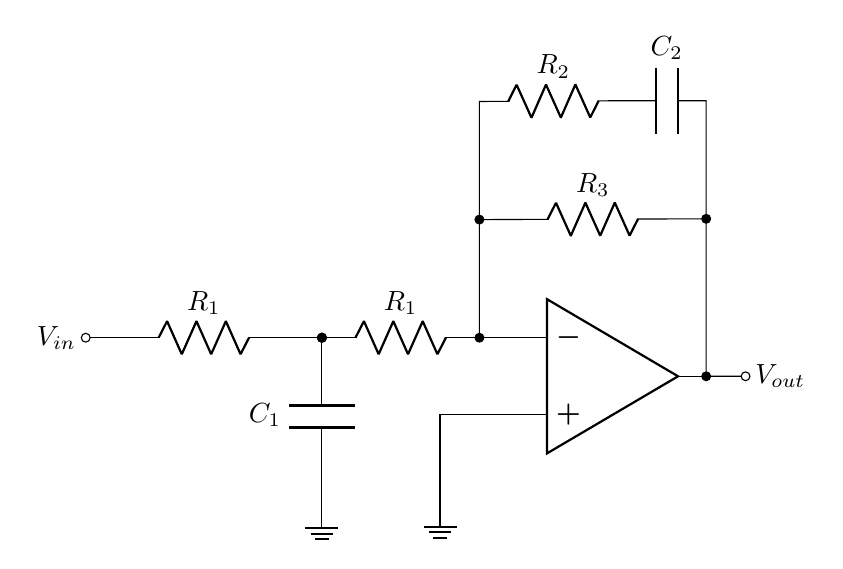
\begin{tikzpicture}
	\node[op amp, yscale=1] (opamp) at (6,-0.5) {};
	\draw ($(opamp.-)+(-5.5,0)$) node[left] {$V_{in}$} 
	to[R, l=$R_1$, o-*] ($(opamp.-)+(-2.5,0)$) node (nodebetween1) {}
	to[R, l=$R_1$, *-*] ($(opamp.-)+(-0.5,0)$) node (nodebetween2) {}
	to[short] (opamp.-);
	\draw (nodebetween1.center) to[C, l_=$C_1$, *-] ($(nodebetween1)+(0,-2)$) node [ground] {};
	\draw (nodebetween2.center) to[short] ($(nodebetween2.center)+(0,1.5)$) to [R, l=$R_3$, *-*] ($(opamp.out)+(0,2)$) 
    to[short] (opamp.out);
    \draw ($(nodebetween2.center)+(0,1.5)$) to[short] ($(nodebetween2.center)+(0,3)$) to [R, l=$R_2$,-] ($(opamp.out)+(-1,3.5)$)
    to [C, l=$C_2$,-] ($(opamp.out)+(0,3.5)$) 
	to[short]  ($(opamp.out)+(0,2)$) ;
	%\draw (nodebetween4.center) to[C, l=$C_2$, *-] ($(nodebetween4.center)+(0,-3)$);
	\draw ($(opamp.+)$) to ($(opamp.+)+(-1,0)$) to ($(opamp.+)+(-1,-1)$) node [ground] {};
	\draw (opamp.out) to[short, *-o]  ($(opamp.out)+(0.5,0)$) node[right] {$V_{out}$};
\end{tikzpicture}
\end{document}